\documentclass{beamer}
\usepackage{beamerthemesplit}
\usepackage{wrapfig}
\usetheme{SPbGU}
\usepackage{pdfpages}
\usepackage{amsmath}
\usepackage{mathtools}
\usepackage{cmap}
\usepackage{indentfirst}
\usepackage{tikz}
\usepackage{multirow}
\usepackage[noend]{algpseudocode}
\usepackage{algorithm}
\usepackage{algorithmicx}
\usepackage{stmaryrd}
\usepackage{fancyvrb}
\usepackage{qtree}
\usepackage{verbatim}
\usepackage{ulem}
\usepackage{proof}
\usepackage{mathtools}
\usepackage{ulem}
\usepackage{listings}
\usepackage{color}
\usepackage{pifont}% http://ctan.org/pkg/pifont
\newcommand{\cmark}{\ding{51}}%
\newcommand{\xmark}{\ding{55}}%

\newcommand{\wbigcup}{\mathop{\bigcup}\displaylimits}
\newcommand{\wbigsqcup}{\mathop{\bigsqcup}\displaylimits}

\beamertemplatenavigationsymbolsempty

\setbeamertemplate{itemize item}[circle]
\setbeamertemplate{enumerate item}[circle]
\newcommand{\derives}[1][*]{\xRightarrow[]{#1}}

\def\To{\derives[]}
\def\iff{\Leftrightarrow}

\usetikzlibrary{shapes,arrows}
\usetikzlibrary{positioning,automata}
\tikzset{every state/.style={minimum size=0.2cm},
initial text={}
}

\graphicspath{
  {pics/}
}

\newcommand{\incimage}[2][0.8]{
  \begin{center}
    \includegraphics[width=\textwidth, height=#1\textheight, keepaspectratio]{#2}
  \end{center}
  }

\title[]{Mode System in Mercury}
\subtitle[]{}
\institute[]{JetBrains Programming Languages and Tools Lab
}

\author[]{Kate Verbitskaia}

\date{30.08.2022}

\definecolor{orange}{RGB}{179,36,31}

\begin{document}
{
  \begin{frame}
    \titlepage
  \end{frame}
}

\begin{frame}[fragile]
  \frametitle{Mercury}
\begin{itemize}
  \item Purely declarative: predicates and functions do not have non-logical side effects
  \item Uses powerful static analyses for compilation
  \begin{itemize}
    \item Strong type system
    \item Strong mode system
    \item Strong determinism system
  \end{itemize}
  \item Is intended for real-world use
  \begin{itemize}
    \item Has a module system
    \item Supports higher-order programming, with closures, currying, and lambda expressions
    \item Very efficient
  \end{itemize}
\end{itemize}

\vfill

\url{https://www.mercurylang.org/about.html}

\end{frame}

\begin{frame}[fragile]
  \frametitle{Example Program}
\begin{itemize}
  \item Code
  \item See also: \url{https://github.com/Mercury-Language/mercury/tree/master/samples}
\end{itemize}
\end{frame}

\begin{frame}[fragile]
  \frametitle{Modes}
  \begin{itemize}
    \item Describe how instantiatedness of variables changes during execution
    \item Basic modes
    \begin{itemize}
      \item \texttt{in == ground >> ground}
      \item \texttt{out == free >> ground}
    \end{itemize}
    \item Modes with extra uniqueness information
    \begin{itemize}
      \item \texttt{di == unique >> clobbered}
      \item \texttt{uo == free >> unique}
    \end{itemize}

  \end{itemize}

\vspace{0.5cm}

  \begin{center}
    \texttt{:- pred append(in, in, out) is det.}
  \end{center}
\end{frame}


\begin{frame}[fragile]
  \frametitle{Benefits of Mode Analysis}
\begin{itemize}
  \item Predicates are specialized according to the mode
  \begin{itemize}
    \item Specialized unifications
    \item Conjunction reordering
  \end{itemize}
  \item No need for occurs check
  \item Early bug detection
  \item Documentation
\end{itemize}
\end{frame}

\begin{frame}[fragile]
  \frametitle{Discriminated Union Types}

\begin{lstlisting}
:- type employee
        ---> employee( name        :: string,
                       age         :: int,
                       department  :: string).

:- type tree
        ---> empty
        ;    leaf(int)
        ;    branch(tree, tree).

:- type list(T)
        ---> []
        ;    [T | list(T)].
\end{lstlisting}

\end{frame}

\begin{frame}[fragile]
  \frametitle{Instantiatedness Declarations}
\begin{center}
  Assigning either \texttt{free} or \texttt{bound} to nodes of a type tree
\end{center}

\begin{lstlisting}[]
:- type list(T) ---> []; [T | list(T)].

:- inst listskel == bound([] ; [free | listskel]).

:- inst listskel(Inst) for list/1
   ---> []
   ;    [Inst | listskel(Inst)]
\end{lstlisting}

\begin{center}
Terms approximated with instantiatedness \texttt{listskel}

\end{center}

\begin{itemize}
  \item[\cmark] \texttt{[A, B]}
  \item[\xmark] \texttt{[A, 2]}
  \item[\xmark] \texttt{[H | T]}
  \item[\xmark] \texttt{[A, A]}
\end{itemize}
\end{frame}


\begin{frame}[fragile]
  \frametitle{Mode Correctness: High Level Idea}
\begin{center}
  A variable cannot become more free after predicate execution
\end{center}

\vfill

Precise and expressive mode systems for typed logic programming languages.
David Overton (PhD thesis): \url{https://mercurylang.org/documentation/papers.html#dmo-thesis}
\end{frame}

\begin{frame}[fragile]
  \frametitle{Instantiation State}
$$
  \iota ::= free \mid bound(\mathcal{P} f (\overline{\iota}))
$$

\end{frame}

\begin{frame}[fragile]
  \frametitle{Mode Annotations for \texttt{append(in, in, out)}}
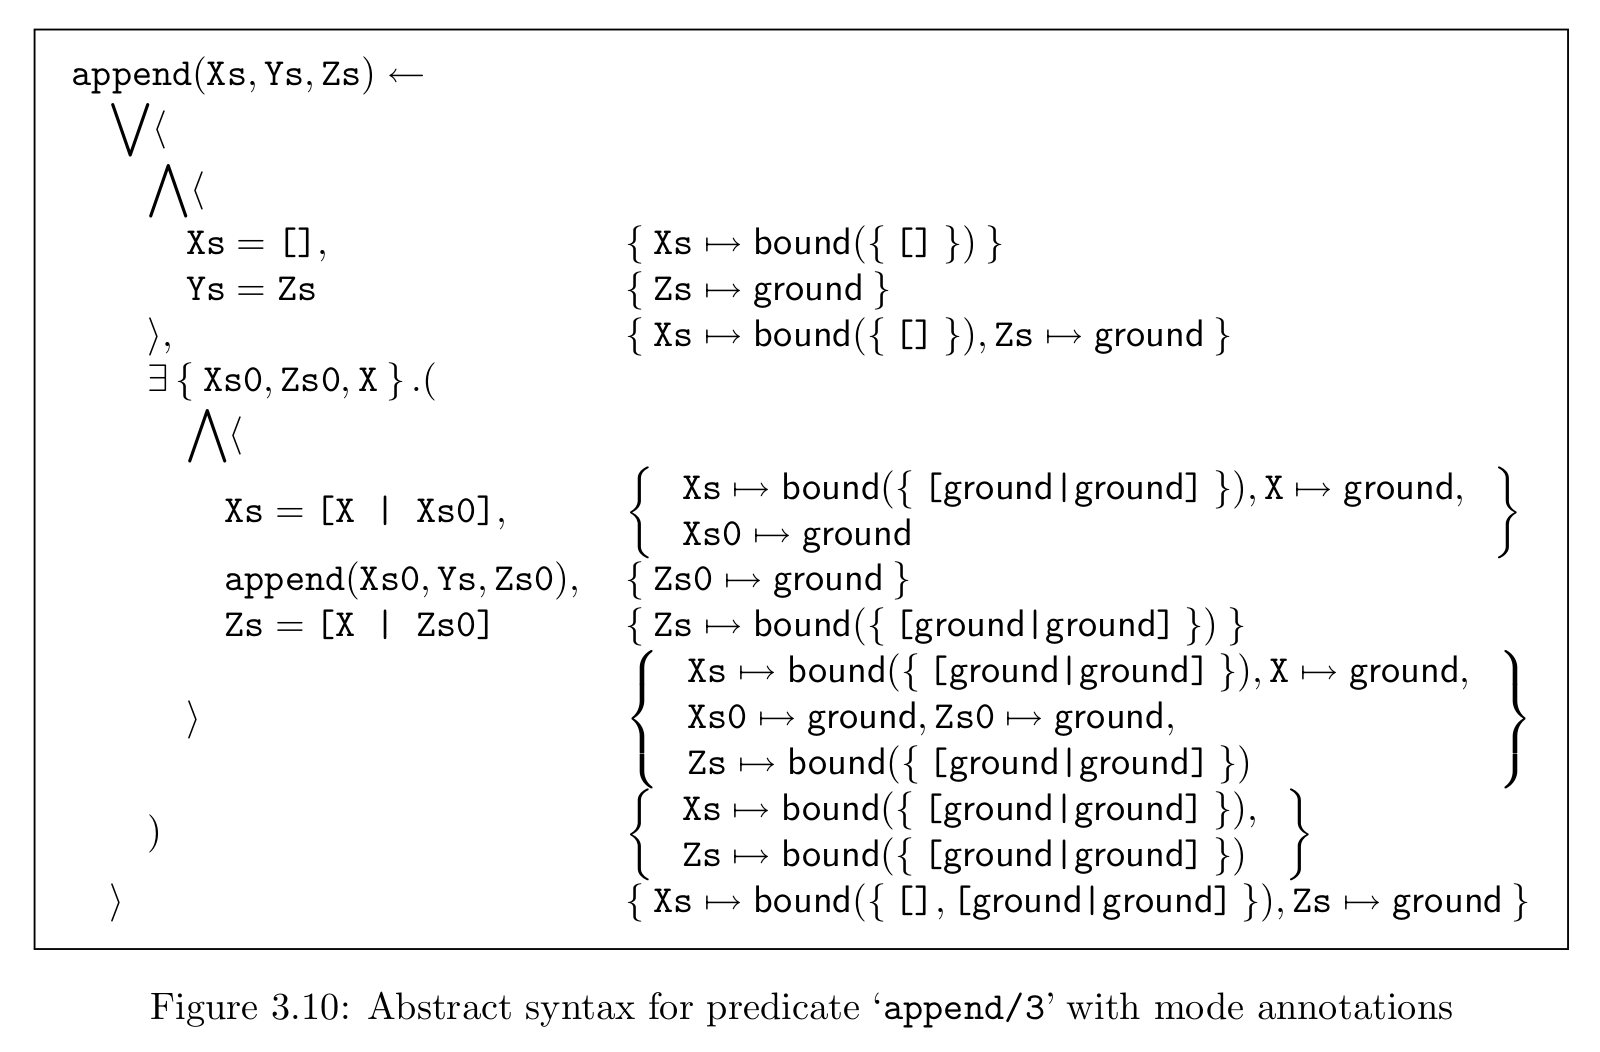
\includegraphics[width=\textwidth]{ModeAnnot.png}
\end{frame}

\begin{frame}[fragile]
  \frametitle{Partial Order on Insts}
  $$
  \iota \preceq free
  $$

  \vfill

  $$
  bound(B) \preceq bound(B') \ iff
  $$
  $$
  \forall \beta \in B. \exists \beta' \in B'. \beta = f (\iota_1, \dots, \iota_n), \beta' = f (\iota_1', \dots, \iota_n'), \forall i. \iota_i \preceq \iota_i'
  $$

  \vfill

  $$
  not\_reached = bound(\varnothing)
  $$
\end{frame}

\begin{frame}[fragile]
  \frametitle{Partial Order Example}
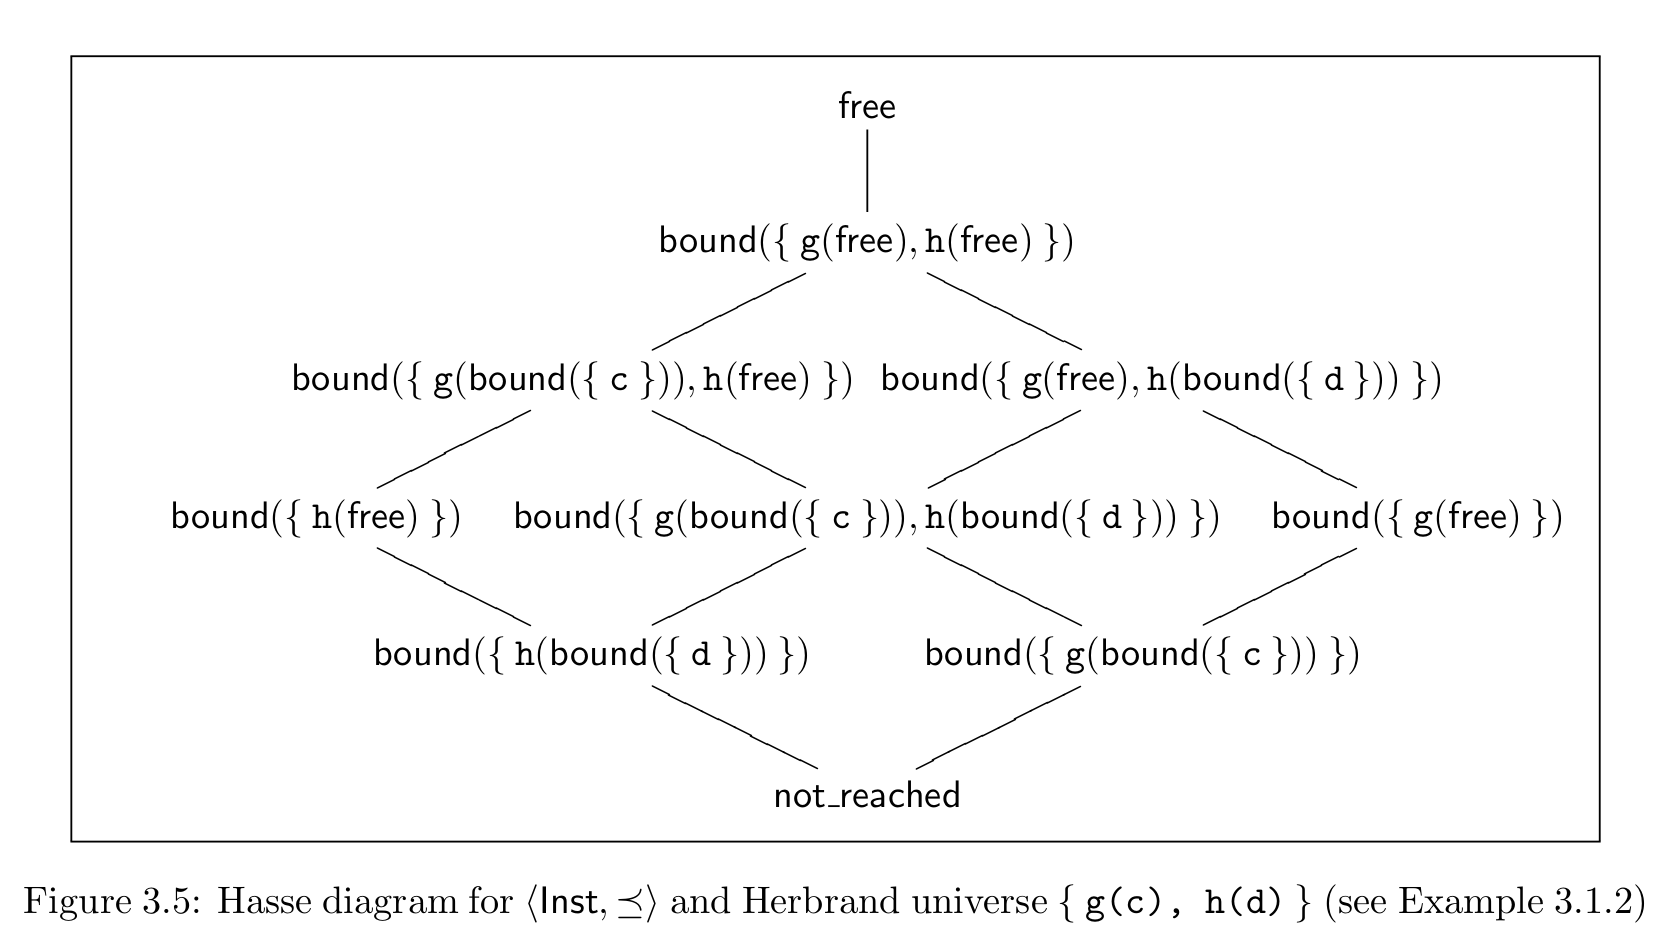
\includegraphics[width=\textwidth]{pics/InstsPO.png}
\end{frame}

\begin{frame}[fragile]
  \frametitle{Insts Concretization}
  $$
  \gamma(free) = \{ \_ \}
  $$

  $$
  \gamma(bound(B)) = \wbigcup_{f(\iota_1, \dots, \iota_n) \in B} \{ f(t_1, \dots, t_n), \forall j. t_j \in \gamma(\iota_j)\}
  $$
\end{frame}

\begin{frame}[fragile]
  \frametitle{Matches Partial Order}
  $$
  free \sqsubseteq free
  $$

  \vfill

  $$
  not\_reached \sqsubseteq free
  $$

  \vfill

  $$
  bound(B) \sqsubseteq bound(B') \ iff
  $$
  $$
  \forall \beta \in B. \exists \beta' \in B'. \beta = f (\iota_1, \dots, \iota_n), \beta' = f (\iota_1', \dots, \iota_n'), \forall i. \iota_i \sqsubseteq \iota_i'
  $$

  \vfill

  $$
  not\_reached = bound(\varnothing)
  $$
\end{frame}

\begin{frame}[fragile]
  \frametitle{Matches Partial Order Example}
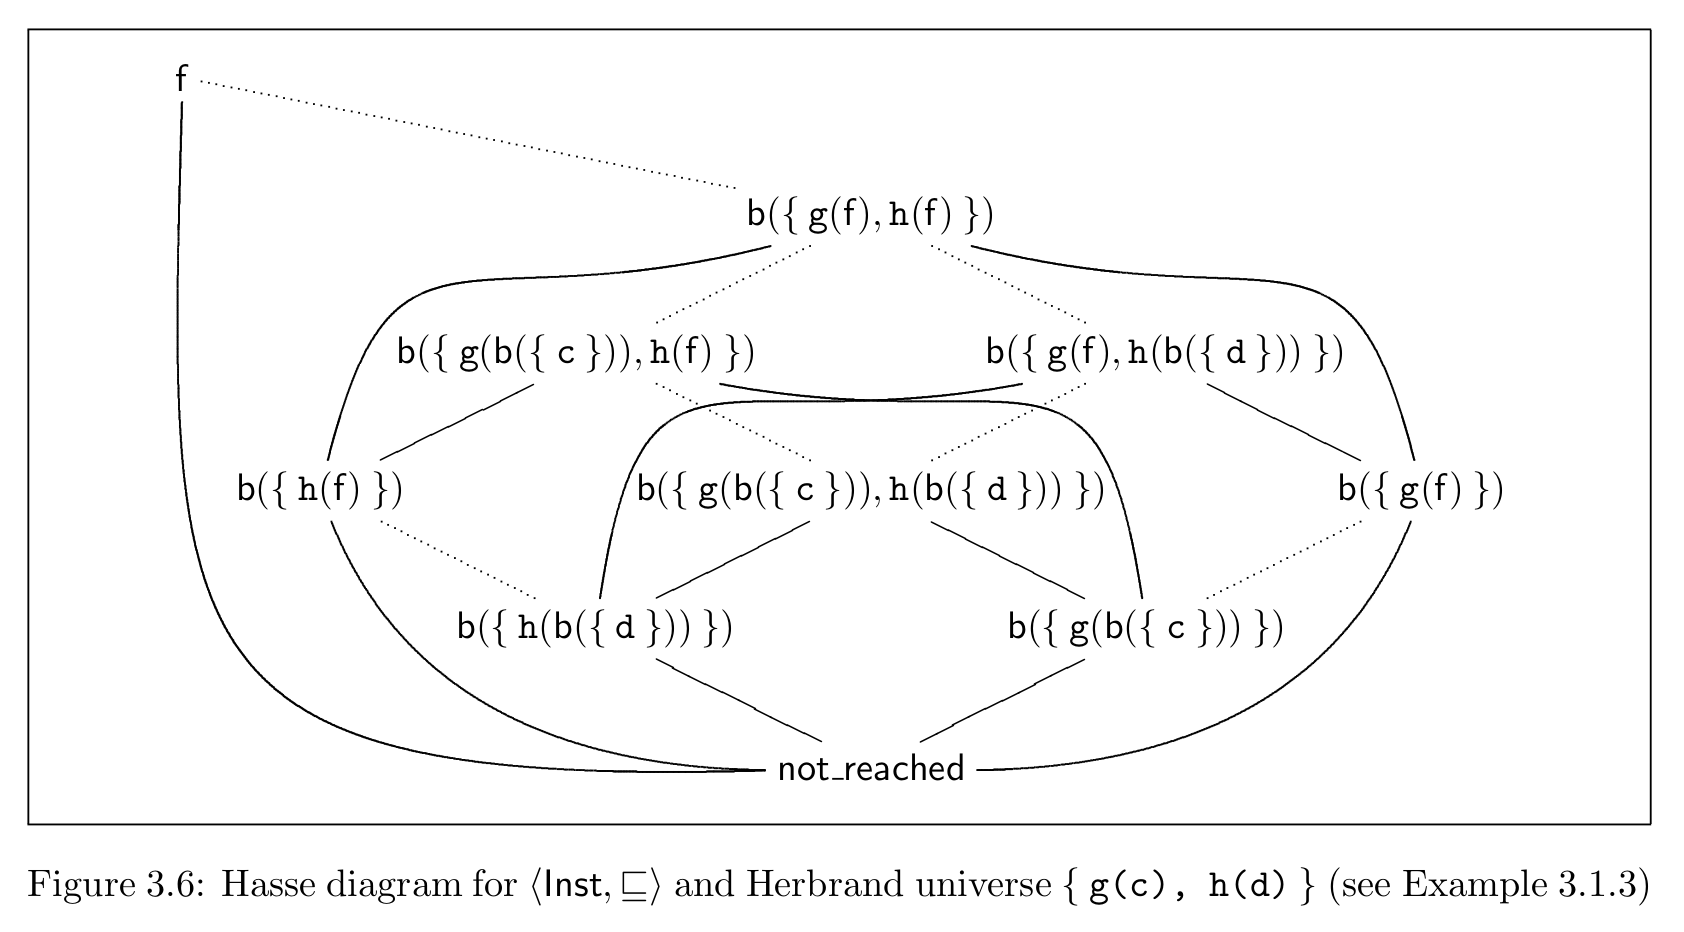
\includegraphics[width=\textwidth]{pics/MatchesPO.png}
\end{frame}

\begin{frame}[fragile]
  \frametitle{Terms Abstraction}
$$
\alpha(T) = \wbigsqcup_{t \in T} \{ \alpha'(t) \}
$$

$$
\alpha'(\_) = free
$$

$$
\alpha'(f(t_1, \dots, t_n)) = bound(\{f(\alpha'(t_1), \dots, \alpha'(t_n))\})
$$
\end{frame}


\begin{frame}[fragile]
  \frametitle{Mode Checking Algorithm}
\begin{itemize}
  \item To mode check the program, mode check all predicates
  \item To mode check a predicate:
  \begin{itemize}
    \item Initialize insts of head vars with initial insts
    \item Mode check the body goal
    \item If no mode errors, check that final insts match the final insts declaration
  \end{itemize}
\end{itemize}
\end{frame}

\begin{frame}[fragile]
  \frametitle{Mode Checking: Disjunction}
  \begin{itemize}
    \item Mode check each disjunct
    \item Merge resulting insts
    $$
    merge(\langle I, I' \rangle, \langle I, I'' \rangle) = \langle I, \{ v \to \iota \mid v \in dom(I) \wedge \iota = I'(v) \sqcup I''(v) \}\rangle
    $$
  \end{itemize}

\end{frame}

\begin{frame}[fragile]
  \frametitle{Mode Checking: Conjunction}
  \begin{itemize}
    \item Schedule a conjunct if possible
    \begin{itemize}
      \item Scheduling: attempt to mode check
      \begin{itemize}
        \item If success, then scheduling succeeds and we commit to the current order
        \item If fails with not sufficiently instantiated local variable, check other order
      \end{itemize}
      \item Delay conjunct if its not sufficiently instantiated
      \item Every time a var is bound, check if a delayed conjunct should be awakened
    \end{itemize}
    \item Mode check conjuncts, combine the result
    $$
    combine(\langle I, I' \rangle, \langle I', I'' \rangle) = \langle I, I'' \rangle
    $$
  \end{itemize}

\end{frame}


\begin{frame}[fragile]
  \frametitle{Reordering of Conjuncts}
\begin{itemize}
  \item Conjunction may be not mode-correct, but some permutation of conjuncts may be
  \item Mode checker may pick any mode-correct permutation
  \item Efficiency not guaranteed
\end{itemize}
\end{frame}


\begin{frame}[fragile]
  \frametitle{Mode Checking: Unification}
  \begin{itemize}
    \item Check that unification does not attempt to unify two free vars
    \item Split unifications to avoid complex unifications
    \item The result inst is the initial inst, but the affected vars are associated with the result of abstract unification:
    $$
    abstract\_unify\_inst(\iota_1, \iota_2, \iota) \ iff \ \iota = \iota_1 \curlywedge \iota_2 \wedge \iota \curlywedge ground
    $$
  \end{itemize}
\end{frame}

\begin{frame}[fragile]
  \frametitle{Mode Checking: Call}
  \begin{itemize}
    \item Check that there is a mode which matches the insts of args
    \item If there is none, attempt to infer mode
    \item !NB Modes may be implied
    \begin{itemize}
      \item{\cmark} append(in, in, in) is an implied mode of append(in, in, out)
      \item{\xmark} append(out, in, in) is not an implied mode of append(in, in, out)
    \end{itemize}
  \end{itemize}
\end{frame}


\begin{frame}[fragile]
  \frametitle{Mode Inference}
\begin{itemize}
  \item Set init insts
  \item Set final insts to be \texttt{not\_reached}
  \item Until fix point is reached (final insts)
  \begin{itemize}
    \item Mode check the body goal
    \item Normalize final insts
  \end{itemize}
\end{itemize}
\end{frame}


\begin{frame}[fragile]
  \frametitle{What is Not in this Talk}
\begin{itemize}
  \item Determinism Analysis
  \item Uniqueness and liveness
  \item Polymorphism
  \item Constraint-based mode analysis
\end{itemize}

\end{frame}

\end{document}